\documentclass{beamer}
\mode<presentation>
\usepackage[czech]{babel}
\usepackage[latin2]{inputenc}
\usepackage[T1]{fontenc}

\usepackage{picture}

\usetheme{Madrid}

\subtitle{Projekt do p�edm�tu SFC}
\title{Demonstrace u�en� s�t� RCE}
\author{Petr Kub�t, xkubat11}
\institute[FIT VUT] {FIT VUT Brno}
\date{\today}

\begin{document}

\begin{frame}
\titlepage
\end{frame}

\section{Detaily projektu}
\begin{frame}
	\frametitle{Detaily projektu:}
	\begin{itemize}
		\item Implementa�n� jazyk: C++
		\item Algoritmus p�evzat� z p�edn�ek
		\item Textov� vstup (soubor) i v�stup
		\item Jednoduch� klasifik�tor po nau�en�
	\end{itemize}
\end{frame}

\section{Vstupn� data}
\begin{frame}
	\frametitle{Vstupn� data}
    \begin{columns}
        \begin{column}{0.5\textwidth}
            \begin{itemize}
                \item Vstup ze souboru
                \item N-rozm�rn� vektor a t��da
                \item Vektory zpracov�v�ny postupn�, nen�hodn�
                \item Max. polom�r pomoc� argumentu -r
            \end{itemize}
        \end{column}
        \begin{column}{0.4\textwidth}
            \begin{block}{Dvourozm�rn� vektory}
                \begin{columns}[totalwidth=\textwidth]
                    \begin{column}{0.5\textwidth}
                        \centering
                        \fontsize{9}{9}\selectfont
                        1 0 0 \\
                        2 0 0 \\
                        3 0 1\\
                        2 1 0\\
                        6 0 1\\
                        7 0 1\\
                        1 8 2\\
                        2 8 2
                    \end{column}
                    \begin{column}{0.5\textwidth}
                        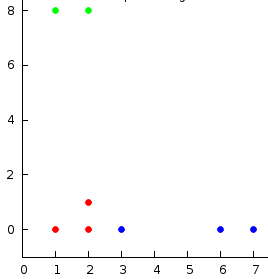
\includegraphics[scale=0.25]{input.png}
                    \end{column}
                \end{columns}
            \end{block}
        \end{column}
    \end{columns}
\end{frame}

\section{V�stup}
\begin{frame}\frametitle{V�stup aplikace}
\begin{center}
    \fontsize{9}{9}\selectfont
    \begin{columns}
        \begin{column}{0.5\textwidth}
            U�en� s�t� \\
            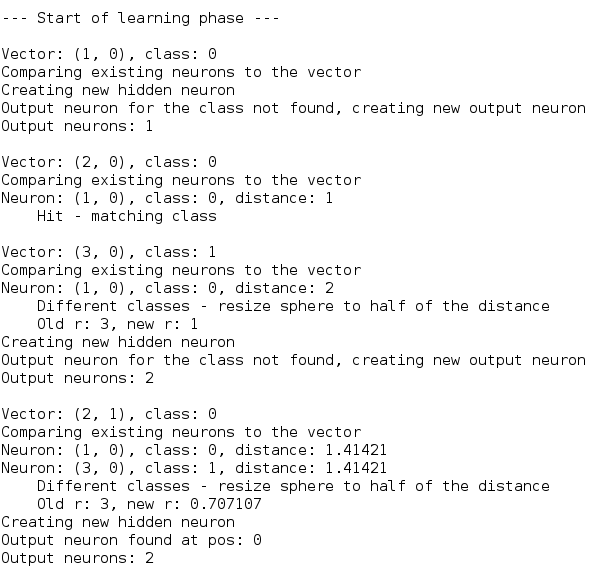
\includegraphics[scale=0.25]{output_learning.png}
        \end{column}
        \begin{column}{0.5\textwidth}
            V�sledn� s�� \\
            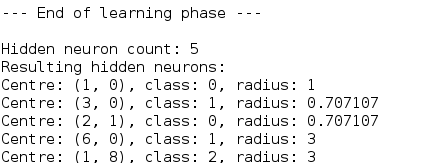
\includegraphics[scale=0.25]{output_link.png} \\
            Vizualizace v�sledku \\
            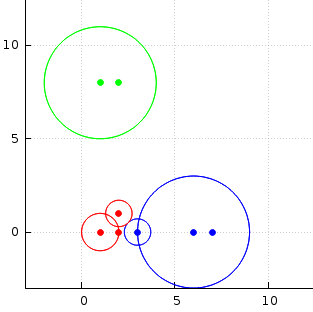
\includegraphics[scale=0.25]{output_grafic.png}
        \end{column}
    \end{columns}
\end{center}
\end{frame}



\end{document}
